\begin{frame}{Agenda}
	\begin{columns}[T]
		\begin{column}{.4\textwidth}
% 			\begin{block}{Your textblock}
				\begin{itemize}
				    \item Motivation: \emph{Landunter} im Stollen!
				    \begin{itemize}
							\item[\to] Das Erbe des Bergbaus
					\end{itemize}
				    \item Lösung: Myonen als "Röntgenstrahlung"
				    \begin{itemize}
				            \item Das Prinzip der Myographie
							\item[\to] Pyramiden, Vulkane und Bergbau 
					\end{itemize}
					\item Myographie im Ruhrgebiet
				    \begin{itemize}
							\item Wie lässt sich ein Wasserpegel untertage messen?
				    		\item Detektor-Zählraten simulieren
				    		\item Ein Bodenprofil im Ruhrgebiet
					\end{itemize}
					
				\end{itemize}
% 			\end{block}
		\end{column}
		\begin{column}{.5\textwidth}
% 			\begin{block}{Your image}
                %% allgemeines cooles myographie bild
				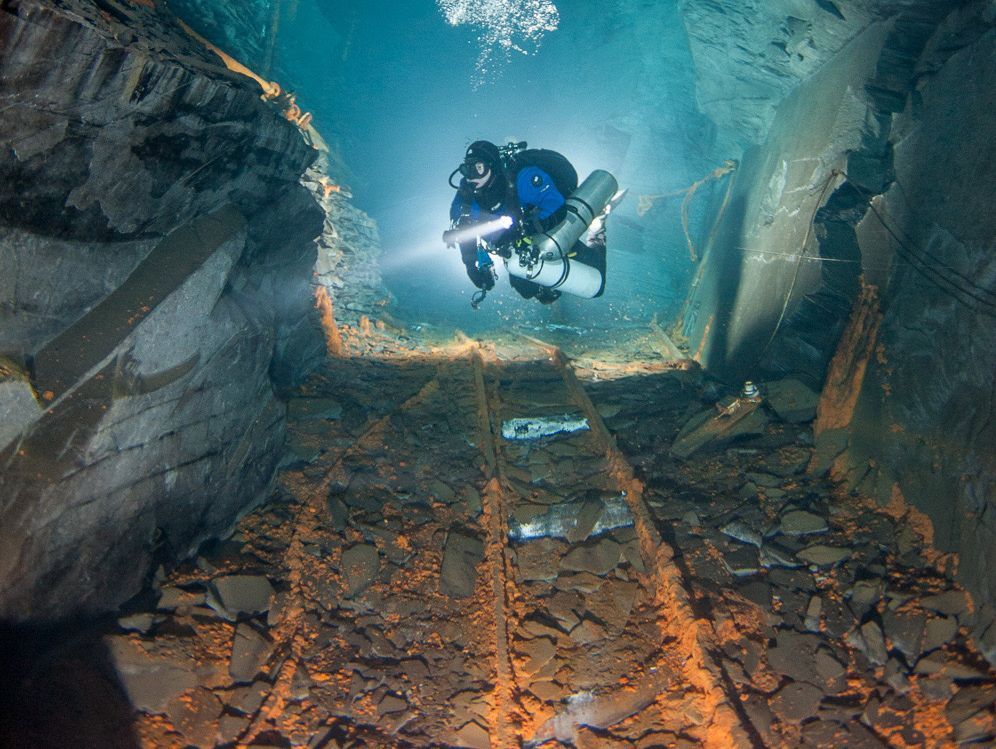
\includegraphics[width=\textwidth]{images/wasser_stollen.jpg}
				\raggedleft{\footnotesize{\href{https://www.spiegel.de/reise/deutschland/bergwerk-nuttlar-in-bestwig-tauchen-mit-tunnelblick-a-914935.html}{[Spiegel - uwpics-bjoern.de]}}}
% 			\end{block}
		\end{column}
	\end{columns}
\end{frame}